\chapter{$\lhcb$实验上$\psitwos$的微分产生截面测量}
\section{选题动机}

质心能量为7$\tev$ $\pp$对撞下,$\lhcb$上已经对$\psitwos$ 的微分产生截面进行过了研究~\cite{Khachatryan:2015rra}。13 $\tev$ $\pp$对撞下,对其微分产生截面进行重新测量,不仅可以更好的检验理论模型,还可以很好的了解微分产生截面随质心能量的变化,并且足够大统计量的$\psitwos$介子可使得微分产生截面的测量精度更高。鉴于$\psitwos$ 在粲偶素家族中处于激发态而不是基态位置,使得受到来自feed-down部分的影响可以忽略,其结果与理论比较更加容易。

\section{$\lhc$和$\lhcb$简介}
\label{sec:lhcb}
本章所研究的$\psitwos$介子是由$\pp$对撞机制产生的,对撞时发生的物理过程的相关信息,目前只能由探测器来收集。
为详细了解$\psitwos$介子的来源,本章先简要介绍高能质子—质子($\pp$)对撞的加速器$\lhc$(Large Hadron Collider) 和该加速器上专门用来研究$b$物理的探测器$\lhcb$(The Large Hardon Collider beauty experiment) 实验。

\subsection{$\lhc$简介}
$\lhc$是一个环形的质子-质子对撞机,前身是欧洲核子中心原有的大型正负电子对撞机(Large Electron Positron collider, LEP)。
$\lhc$实际上是一个加速器链的最后一环,其隧道周长约为26.7千米,整个加速器综合体如图~\ref{fig:lhc} 所示。
\begin{figure}
\begin{center}
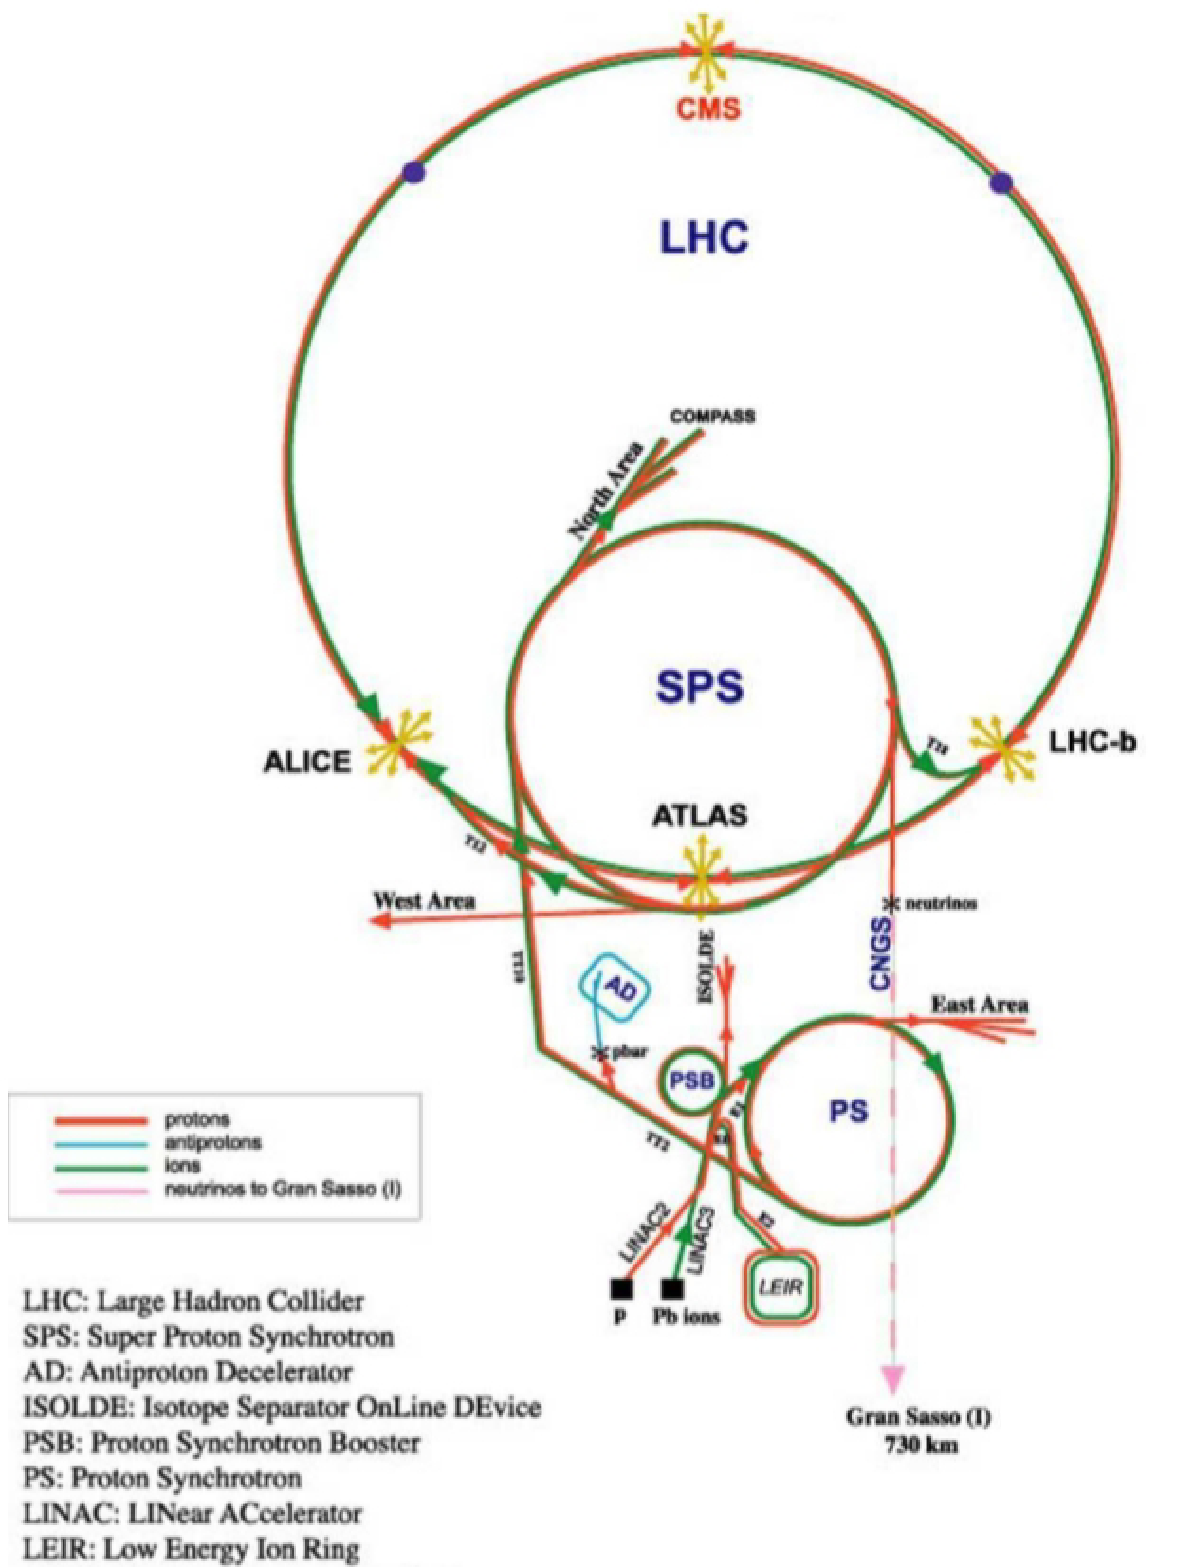
\includegraphics[width=0.9\textwidth]{chap3_lhc}
\caption{$\lhc$及其附属装置示意图。}
\label{fig:lhc}
\end{center}
\end{figure}

$\lhc$中质子的加速是被安排成束团(bunch)来进行的,每个束团大概包含$10^{11}$ 个质子,两个束团交叉的时间间隔为25 ns,为了将这些束团限制在$\lhc$ 环形轨道上,采用了由Nb-Ti超导磁铁提供的约为8.33特斯拉的扭转磁场。在加速器链中,质子产生后经过直线加速器(LINAC)、质子同步加速器(Proton Synchrotron, PS)、质子同步加速升压器(Proton Synchrotron Booster, PSB)、超级质子同步加速器(Super Proton Synchrotron, SPS)相继被加速到450 $\gev$,随后质子被分成两束,在$\lhc$ 加速腔体内的不同束流管中相向被加速到6 $\tev$,最终两束质子对撞时的质心能量为13 $\tev$。 表~\ref{tab:lhc}是$\lhc$ 的部分设计参数。
\begin{table}
\centering
%\footnotesize
\caption{$\lhc$的部分设计参数。}
\begin{tabular}{ll}
\toprule
周长                                 & 26.7 km\\
注入能量                             & 0.45 $\tev$  \\
设计亮度                             & $10^{34} \rm{cm}^{-2}s^{-1}$ \\
亮度寿命                             & 10 h \\
束流寿命                             & 22 h \\
束团间隔                             & 25 ns\\
束团中质子数                         & $1.15\times10^{11}$ \\
储存束流能量                         & 334 MJ\\
质子运行一圈损失能量                 & 7.6 eV \\
每束束流辐射能量                     & 3.6 kw\\
\bottomrule
\end{tabular}
\label{tab:lhc}
\end{table}

\subsection{$\lhcb$装置简介}

标准模型中弱相互作用给出的CP破坏尺度太小而不能对宇宙中正反物质的不对称性给出满意的解释。
因此,需要用标准模型或超出标准模型的CP破坏的新来源去解决问题。
$\lhcb$是一个单臂前向探测器,作为$\lhc$上重点研究重味物理的实验,最初的设计目标是利用高统计量优势更高精度去测量标准模型参数,研究$b$物理和$c$物理中的CP 破坏和稀有衰变,为新物理提供间接证据。
另外,$\lhcb$上高统计量的实验数据使得在重味物理中寻找CP破坏新的来源成为可能。
并且13 $\tev$下更高的$c\overline{c}$ 微分截面和$b\overline{b}$微分截面,使得$\lhcb$实验成了最丰富的$c$强子和$b$强子来源。
$\lhcb$探测器总体具有好的顶点位置分辨率、好的固有时间分辨率、好的动量分辨率、好的粒子鉴别能力,以及在其几何接受度范围内物质尽可能少,从而减少多级散射带来的影响。$\lhcb$探测器装置示意图如~\ref{fig:detector}所示。

\begin{figure}
\begin{center}
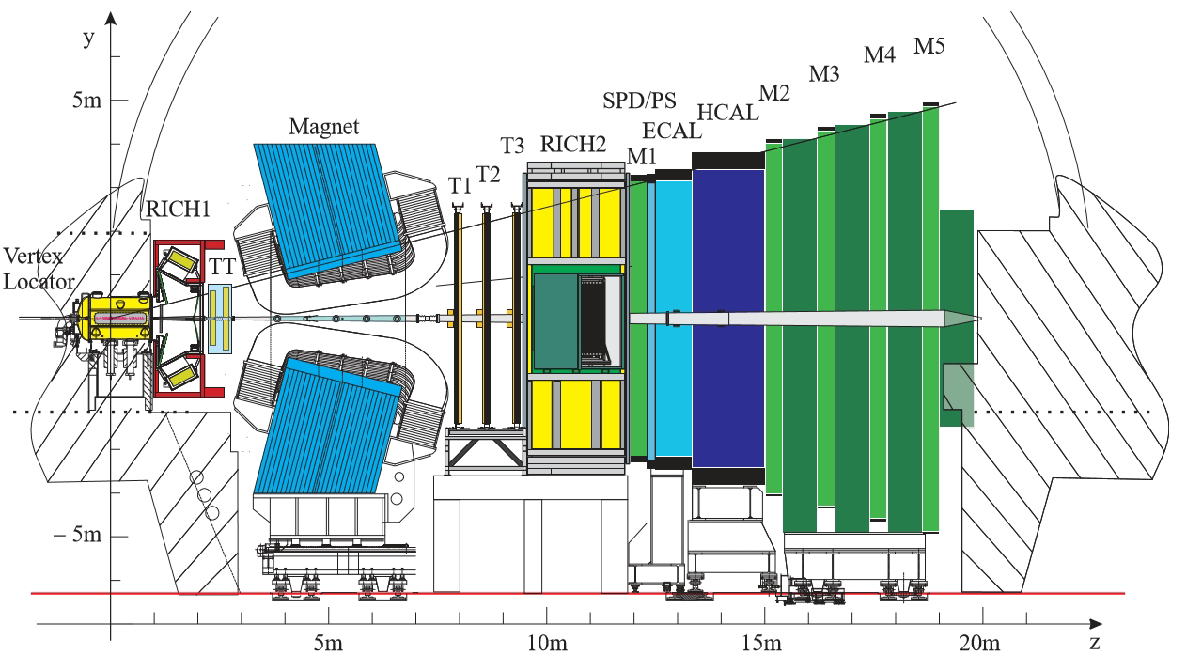
\includegraphics[width=0.9\textwidth]{chap3_lhcb}
\caption{$\lhcb$探测器装置示意图。}
\label{fig:detector}
\end{center}
\end{figure}

\subsection{$\lhcb$数据处理框架}
$\lhcb$软件采用的是基于面向对象的Gaudi框架。
$\lhcb$的应用程序包括事例产生、探测器模拟、数字化、重建、触发、物理分析和事例及探测器显示等,都是在Gaudi框架中来完成它们的任务。Gaudi的一大特色是数据处理的算法部分被当成对象来处理,对应用程序在运行时进行设置,是Gaudi提供的一个重要服务作业选项服务,它通过和成分的数据成员(如算法)相关联的属性(properties)来进行。基于Gaudi框架的数据处理应用程序和数据流如图~\ref{fig:data_program}所示。
 \begin{figure}
 \begin{center}
 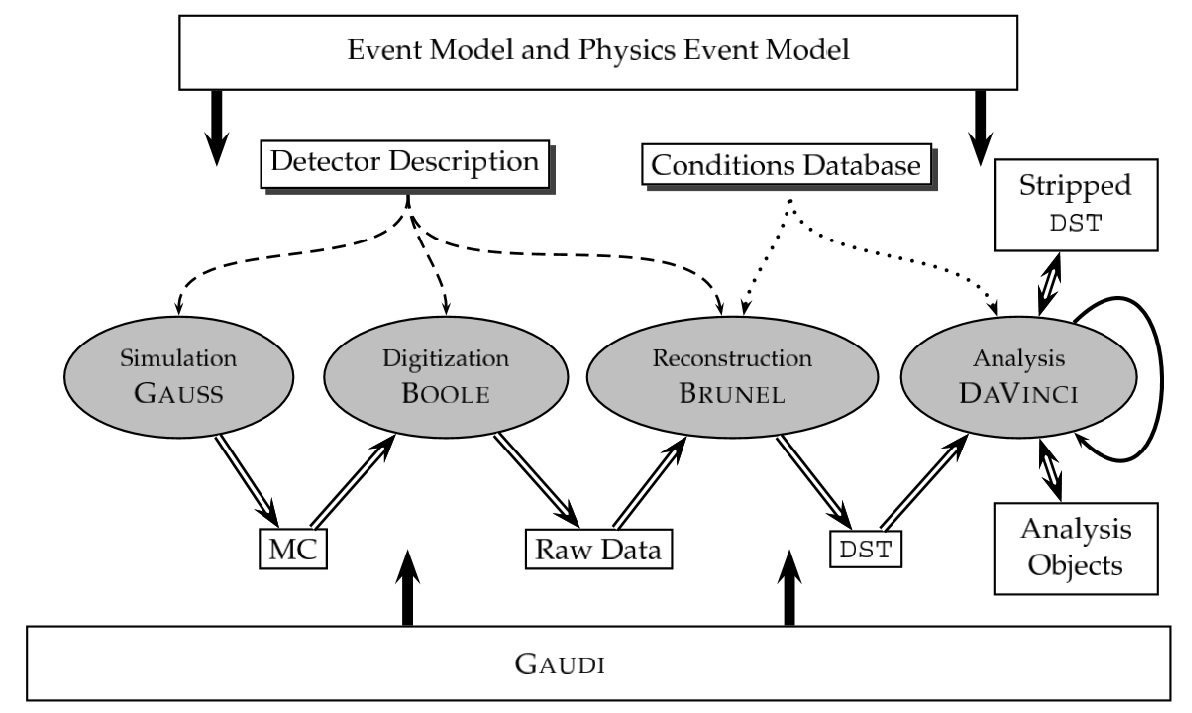
\includegraphics[width=0.8\textwidth]{chap3_data_flow}
\caption{ $\lhcb$数据处理应用程序和数据流。}
\label{fig:data_program}
 \end{center}
\end{figure}
